\chapter{Weryfikacja modelowa}

Systemy tworzone przez ludzi są coraz bardziej złożone oraz zwiększa się ich rola w życiu każdego z nas.
Błędy w oprogramowaniu skutkują stratami finansowymi, wizerunkowymi, opóźnieniami, a także utratą zdrowia i życia ludzi. Dowodzą temu następujące przykłady: nieudany start Ariane-5 (04.06.1996), błąd w procesorach Pentium II Intela, czy źle działająca maszyna do radioterapii, która spowodowała śmierć sześciu pacjentów w latach 1985-1987.


\section{Weryfikacja systemu}

Weryfikacja systemu ma na celu ustalenie, czy projekt zawiera oczekiwane właściwości. Mogą one być podstawowe i niezależne od implementowanej dziedziny (np. nigdy nie dojdzie do zakleszczenia) lub z nią związane (np. nie można wypłacić więcej pieniędzy, niż jest na koncie). Specyfikacja dostarcza informacji, jak system może oraz jak nie może się zachowywać. Oprogramowanie uważa się za poprawne, jeśli spełnia wszystkie właściwości. Schemat weryfikacji został przedstawiony na rys. \ref{fig:system_verification_scheme}.

\begin{figure}[h]
    \centering
    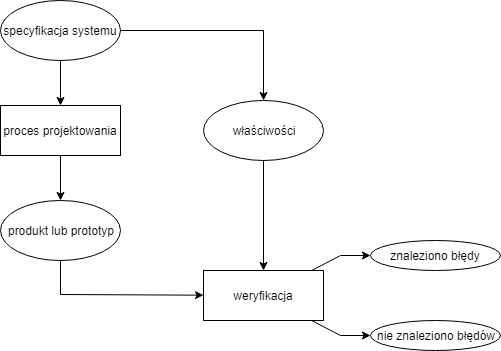
\includegraphics[height=8cm,keepaspectratio]{img/system_verification_schematic_view.png}
    \caption{Schemat tworzenia systemu wraz z jego weryfikacją (źródło~\cite{Bai08}).}
    \label{fig:system_verification_scheme}
\end{figure}

Podstawową formą radzenia sobie z błędami jest testowanie oprogramowania (testy jednostkowe, integracyjne, systemowe itp.).
Proces testowania oprogramowania polega na uruchamianiu skompilowanej całej aplikacji lub jednie poszczególnych jej elementów wraz z wymuszeniem różnych przepływów sterowania, po czym porównuje się rezultaty rzeczywistego działania fragmentu kodu z oczekiwanymi wynikami.
Niestety, przetestowanie wszystkich wariantów w sposób wyczerpujący okazuje się praktycznie niemożliwe, zwykle sprawdzane są je dynie warunki brzegowe, które stanowią mały podzbiór wszystkich potencjalnych kombinacji.

Szczególnym wyzwaniem okazują się testy programów współbieżnych.
Błędy zawarte w takich aplikacjach mogą ujawniać się w specyficznych warunkach.
Zdarza się, że testy działają niedeterministycznie i trudno wyjaśnić czemu dochodzi do ich niepowodzenia co kilka tysięcy uruchomień.
Wynika to zwykle z braku kontroli nad współdzielonym zasobem lub niesynchronizowania pracy wątków działających równolegle.


\section{Weryfikacja modelowa}

Podczas tworzenia skomplikowanych systemów, kładzie się coraz większy nacisk na testowanie poprawności oprogramowania.
Metody formalne mają duży potencjał na tym polu.
Ich wczesna integracja z procesem wytwarzania oprogramowania dostarcza efektywnych technik weryfikacji zadanej specyfikacji.
Intuicyjnie, metody formalne można rozważać jako matematykę stosowaną dla modelowania i analizy systemów informatycznych.
Zapewniają one poprawność z matematyczną dokładnością.

Modelem nazywamy opis mechaniki systemu (zwykle uproszczony), który pozwala utworzyć graf reprezentujący wszystkie stany systemu.
Techniki weryfikacji bazujące na modelu opisują zachowanie systemu deterministycznie i kompletnie.
Samo tworzenie pełnego modelu może wykryć luki lub niespójności w projekcie.
Kolejnym krokiem jest eksploracja stanów systemu.
Dzieje się ona w podejściu ``brute-force`` -- przejrzane zostają wszystkie możliwe scenariusze.
W ten sposób udowadnia się spełnialność właściwości.
Weryfikacji podlega również kolejność zdarzeń w czasie, np. czy system zawsze odpowie na żądania klienta w tym samym porządku, w jakim je otrzymał.

\vspace{0.5cm}
\begin{figure}[h]
    \centering
    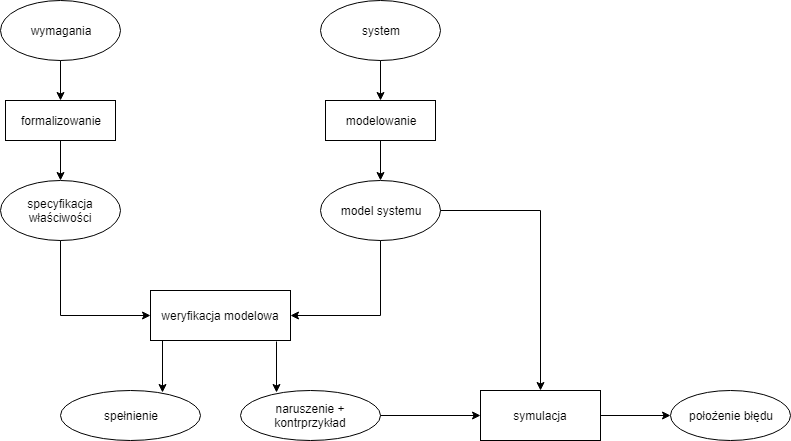
\includegraphics[width=\textwidth,keepaspectratio]{img/model_checking_approach_schematic_view.png}
    \caption{Schemat podejścia weryfikacji modelowej (źródło~\cite{Bai08}).}
    \label{fig:model_checking_scheme}
\end{figure}

\noindent
Kategorie właściwości współbieżnego systemu:
\begin{itemize}
\item osiągalność (niemożliwe jest zakleszczenie)
\item bezpieczeństwo (coś niepożądanego nigdy nie wystąpi \cite{Alp87})
\item żywotność (coś "dobrego" w końcu nastąpi \cite{Alp85})
\item uczciwość (czy przy odpowiednich warunkach zdarzenie występuje powtarzalnie)
\item właściwości czasu rzeczywistego
\end{itemize}

\vspace{0.5cm}
Model systemu zazwyczaj jest generowany automatycznie na podstawie opisu w odpowiednim języku lub dialekcie wspieranym przez narzędzie. 
Weryfikator modelowy przeszukuje kolejne stany.
Następnie sprawdzane są one pod kątem właściwości.
Po znalezieniu naruszenia specyfikacji prezentowany zostaje kontrprzykład, czyli cała ścieżka wykonania, która do niego prowadzi.
Zaprezentowanie kontrprzykładu pozwala lepiej zrozumieć problem, namierzyć źródło niespójności w modelu -- schemat na rys. \ref{fig:model_checking_scheme}.

\vspace{0.5cm}
\noindent
To nie jedyne zalety. Kolejnymi mocnymi stronami weryfikacji modelowej są:
\begin{itemize}
\item Wsparcie częściowej weryfikacji -- możemy sprawdzać poszczególne właściwości niezależnie, nawet gdy pełna specyfikacja nie jest gotowa.
\item To ogólna metoda weryfikacji, która sprawdza się zarówno przy tworzeniu oprogramowania, jak i projektowaniu sprzętu (np. procesorów).
\item Dostarcza informacji diagnostycznych po wykryciu niespełnionej właściwości.
\item Wszystkie możliwe ścieżki wykonania zostają sprawdzone.
\item Uruchomienie weryfikatora nie wymaga ekspertyzy na tym polu, a przynajmniej nie jest znacząco trudniejsze od już szeroko stosowanych testów jednostkowych.
\item Łatwo zintegrować to rozwiązanie z cyklem wytwarzania oprogramowania.
\item Obecnie wzrasta zainteresowanie tym podejściem.
\end{itemize}

\vspace{0.5cm}
\noindent
Oczywiście nie brak także wad:
\begin{itemize}
\item Weryfikowany jest model systemu, a nie sam system. Brak tu gwarancji, że implementacja poprawnie go odtwarza. Model mógł także ulec zbytniemu uproszczeniu.
\item Sprawdzane są tylko wyspecyfikowane wymagania. Nie można wnioskować o poprawności właściwości, których nie ma (błąd niedokładnej specyfikacji \cite{Lam05}).
\item Aplikacje oparte na dużej ilości danych mogą posiadać zbyt wiele stanów, aby weryfikator mógł je wszystkie wygenerować. W ekstremalnych przypadkach liczba stanów może być nieskończona.
\item Podatność na problem eksplozji przestrzeni stanów \cite{Cla11}.
\end{itemize}


\section{Logika LTL}

Logika LTL to jedna z logik temporalnych. Opiera się na liniowej strukturze czasu.
Jej składnia i semantyka pozwala precyzyjnie opisywać bogate spektrum właściwości systemu, włączając w to m.in. bezpieczeństwo czy żywotność \cite{Bel17}.
``Temporalna`` oznacza umiejscawianie zdarzeń relatywnie względem innych, to pewna abstrakcja ponad czasem.  Z tego powodu niewykonalne jest sprawdzenie, czy maksymalne opóźnienie między zdarzeniami wynosi $500ms$.

Formuły LTL ponad zbiorem $AP$ wyrażeń atomowych przedstawia poniższy opis:
\begin{gather}
\varphi::= true \,\, | \,\, false \,\, | \,\, a \,\, | \,\, \neg\varphi \,\, | \,\, \varphi \land \psi \,\, | \,\, \varphi \lor \psi \,\, | \,\, \varphi \Rightarrow \psi \,\, | \,\, \varphi \Leftrightarrow \psi \,\, | \nonumber\\
\mathbf{X}\varphi \,\, | \,\, \mathbf{F}\varphi \,\, | \,\, \mathbf{G}\varphi \,\, | \,\, \varphi\mathbf{U}\psi \,\, | \,\, (\varphi)\nonumber
\end{gather}
gdzie $a \in AP$ \\
Wyjaśnienie symboli (intuicyjna semantyka przedstawiona jest na rys. \ref{fig:ltl_semantics}): \\
$\mathbf{X}$ -- $ne\mathbf{X}t$ -- w następnym stanie \\
$\mathbf{U}$ -- $\mathbf{U}ntil$ -- aż do pewnego momentu w przyszłości \\
$\mathbf{F}$ -- $\mathbf{F}inally$ -- teraz lub w przyszłości \\
$\mathbf{G}$ -- $\mathbf{G}lobally$ -- teraz i w każdym momencie w przyszłości
\vspace{0.5cm}

\begin{figure}[h]
    \centering
    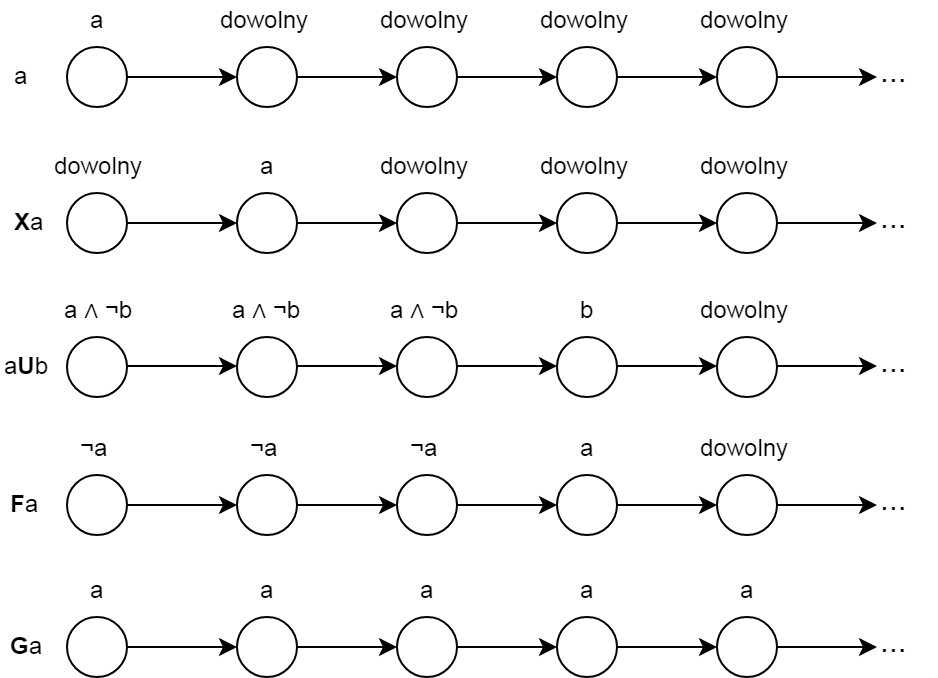
\includegraphics[height=11cm,keepaspectratio]{img/ltl_intuitive_semantics.png}
    \caption{Intuicyjna semantyka temporalnych modalności (źródło~\cite{Bai08}).}
    \label{fig:ltl_semantics}
\end{figure}

Przykładowe formuły LTL:
\begin{itemize}
\item $\mathbf{G}\neg\varphi$ -- niemożliwe jest osiągnięcie stanu posiadającego $\varphi$ (bezpieczeństwo)
\item $\mathbf{G}(\varphi\Rightarrow\mathbf{F}\psi)$ -- dla dowolnego stanu, jeśli posiada on $\varphi$, w końcu znajdziemy stan posiadający $\psi$ (żywotność)
\item $\mathbf{FG}\varphi$ -- w końcu znajdziemy taki stan, od które zawsze spełnione będzie $\varphi$ (stabilność)
\end{itemize}


\section{Automat Büchiego}

W poprzedniej sekcji przedstawiona została logika czasu liniowego LTL.
Niestety w obecnej postaci nie można jej wykorzystać do weryfikacji modelowej.
Punktem startowym jest system tranzycyjny $TS$ oraz formuła LTL $\varphi$, która formalizuje wymaganie dla $TS$.
Zadanie polega na sprawdzeniu, czy $TS \models \varphi$.
Jeśli $\varphi$ jest naruszona, szczegóły błędu powinny zostać dostarczone w postaci sekwencji akcji lub stanów, które prowadzą do naruszenia wymagań. Dostarczona ścieżka ma ułatwić poprawienie modelu i wyeliminowanie błędu.
Manualne dowodzenie $TS \models \varphi$ to zazwyczaj bardzo trudny proces (zwykle systemy tranzycyjne są ogromne).
Dodatkowo rzadkim przypadkiem jest jedna formuła do weryfikacji.
Wymagania składają się najczęściej z całego zbioru wymagań $\varphi_1,...,\varphi_k$.
Wynikają z tego dwie opcje -- można połączyć je w jedną $\varphi_1 \land ... \land \varphi_k$, aby uzyskać specyfikację wszystkich wymagań naraz lub traktować każde wymaganie $\varphi_i$ niezależnie.
Drugie podejście często okazuje się wydajniejsze.
Ponadto znalezienie błędu podczas sprawdzania pełnej specyfikacji nie dostarcza tak precyzyjnych danych diagnostycznych, jak w przypadku gdy wiadomo, która z formuł $\varphi_i$ została niespełniona.

Pomiędzy logiką temporalną a teorią $\omega$-regularnych języków zachodzi bliska relacja \cite{Sis83}\cite{Wol83}.
Języki $\omega$-regularne są analogiczne do regularnych, lecz są zdefiniowane na nieskończonych słowach (zamiast skończonych).
Rozpoznawane są one przez automat Büchiego \cite{Buch66}.
To skończony automat, który operuje na nieskończonych słowach.
Nieskończone słowo jest akceptowane przez automat Büchiego wtedy i tylko wtedy, gdy stan akceptujący wystąpi nieskończenie wiele razy \cite{Sis87}.
Formalnie, deterministyczny automat Büchiego to krotka $A = (Q,\Sigma,\delta,q_0,F)$ składająca się z następujących elementów:
\begin{itemize}
\item $Q$ -- skończony zbiór. Elementy $Q$ nazywane są stanami $A$.
\item $\Sigma$ -- skończony zbiór nazywany alfabetem.
\item $\delta: Q \times \Sigma \rightarrow Q$ -- funkcja nazywana funkcją tranzycji $A$.
\item $q_0$ -- element $Q$, nazywany stanem początkowym $A$.
\item $F \subseteq Q$ -- warunek akceptujący. $A$ akceptuje dokładnie takie przejścia, gdzie przynajmniej jeden z nieskończenie często występujących stanów jest w $F$.
\end{itemize}
W niedeterministycznym automacie Büchiego (NBA -- ang. \textit{non-deterministic Büchi automaton}), funkcja tranzycji $\delta$ zastąpiona jest relacją tranzycji $\Delta$, która zwraca zbiór stanów, a w miejscu stanu początkowego $q_0$ znajduje się zbiór stanów początkowych.

Uogólniony automat Büchiego (GBA -- ang. \textit{generalized Büchi automaton}), to krotka $A = (Q,\Sigma,L,\Delta,Q_0,F)$:
\begin{itemize}
\item $Q$ -- skończony zbiór. Elementy $Q$ nazywane są stanami $A$.
\item $\Sigma$ -- skończony zbiór nazywany alfabetem.
\item $\Delta: Q \times \Sigma \rightarrow 2^Q$ -- funkcja nazywana funkcją tranzycji $A$.
\item $Q_0$ -- podzbiór $Q$, nazywany stanami początkowymi.
\item $F$ -- warunek akceptujący. Składa się z zera lub więcej akceptujących zbiorów. Każdy taki zbiór $F_i \in F$ jest podzbiorem $Q$.
\end{itemize}
Pomimo różnic, GBA to ekwiwalent NBA w kategorii siły ekspresji.
W związku z tym możliwa jest jego konwersja do NBA \cite{Mer14}\cite{Dol95}.

Na rys. \ref{fig:nba1} oraz \ref{fig:nba2} znajdują się przykładowe NBA, wraz z odpowiadającymi im formułami.

\begin{figure}[h]
    \centering
    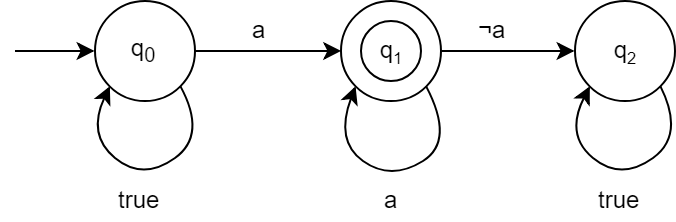
\includegraphics[width=8cm,keepaspectratio]{img/nba1.png}
    \caption{NBA dla $\mathbf{FG}a$ (źródło~\cite{Bai08}).}
    \label{fig:nba1}
\end{figure}
\begin{figure}[h]
    \centering
    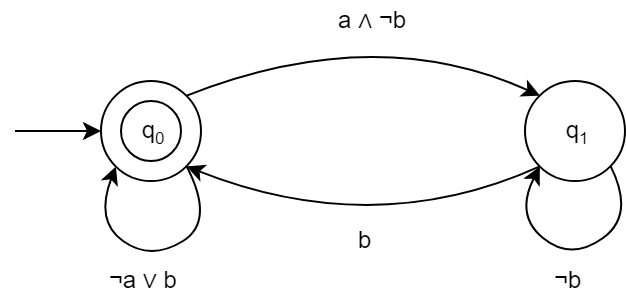
\includegraphics[width=8cm,keepaspectratio]{img/nba2.png}
    \caption{NBA dla $\mathbf{G}(a \Rightarrow \mathbf{F}b)$ (źródło~\cite{Bai08}).}
    \label{fig:nba2}
\end{figure}

\noindent
Algorytm weryfikacji formuły LTL $\varphi$ w systemie tranzycyjnym $TS$ wygląda następująco:
\begin{enumerate}
    \item Zaneguj formułę $\varphi$ otrzymując $\neg\varphi$.
    \item Skonstruuj niedeterministyczny automat Büchiego $A_{\neg\varphi}$ odpowiadający formule $\neg\varphi$.
    \item Skonstruuj wynikowy system tranzycyjny $TS \otimes A$.
    \item Jeśli istnieje ścieżka $\pi$ w $TS \otimes A$ spełniająca akceptujący warunek $A$, zwróć ``nie`` wraz z opisem ścieżki $\pi$, w przeciwnym razie zwróć ``tak``.
\end{enumerate}

\noindent
$TS_1 \otimes TS_2$ -- iloczyn synchroniczny (ang. \textit{synchronous product}) oznacza system tranzycyjny, którego składowe systemy tranzycyjne ($TS_1$ i $TS_2$) wykonują wszystkie akcje synchroniczne, bez ich pomijania przez którykolwiek składowy system tranzycyjny.


Sam schemat przedstawiający jak działa weryfikacja modelowa, kiedy wykorzystujemy logikę LTL do opisu właściwości, znajduje się na rys. \ref{fig:ltl_model_checking}.

\begin{figure}[h]
    \centering
    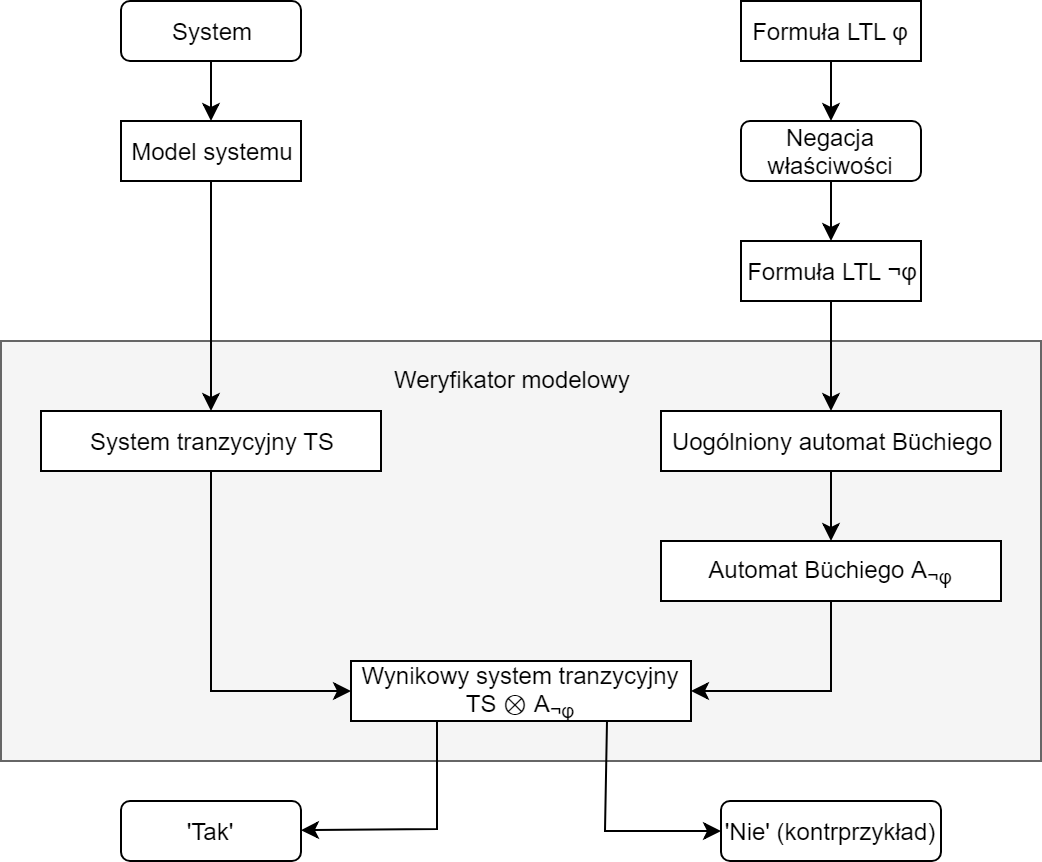
\includegraphics[height=11cm,keepaspectratio]{img/ltl_model_checking_overview.png}
    \caption{Przegląd weryfikacji modelowej LTL (źródło~\cite{Bai08}).}
    \label{fig:ltl_model_checking}
\end{figure}


\section{Eksploracja stanów systemu}

Posiadanie modelu systemu nie oznacza dostępności pełnego grafu stanów.
Może to być niepraktyczne lub nawet niemożliwe ze względu na ich liczbę.
Preferowane podejście to generowanie kolejnych stanów i ich weryfikacja ich w locie, czyli w trakcie ich generacji.
Takie rozwiązanie pozwala na wykrycie niespójności we wczesnym etapie, unikając przeglądania całej przestrzeni stanów.

Kolejnym czynnikiem wpływającym na wydajność jest sam algorytm budujący graf stanów.
W przypadku skomplikowanych systemów spodziewać się można olbrzymiego grafu, więc również czas jego tworzenia będzie odzwierciedlał rozmiar.
Moc obliczeniowa jednego procesora może okazać się niewystarczająca.
Warto więc wykorzystać algorytmy równoległe.
Standardowym rozwiązanie to DFS (przeszukiwanie w głąb -- ang. \textit{Depth-first search}) \cite{God94}\cite{Hol99}.
Występuje w wielu wersjach mających zwiększyć jego wydajność.
Z czasem powstała też nowa grupa algorytmów.
Opiera się na podziale grafu na silnie spójne składowe, wywodzi się ona z algorytmu Tarjana \cite{Jac05}.
Złożoność obliczeniowa tych algorytmów jest liniowa $O(m + n)$, gdzie $m$ to liczba krawędzi, a $n$ oznacza ilość stanów.
Wszystkie korzystają z tej samej zasady eksploracji -- przeszukiwania wstecznego (ang. \textit{post-order}).
Faktem jest, że problem takiego przeszukiwania jest P-zupełny, więc skalowany, równoległy algorytm tego typu prawdopodobnie nie istnieje \cite{Reif85}.

Celem algorytmu weryfikacji modelowej jest eksploracja stanów systemu wraz z synchronicznym wykonywaniem tranzycji w automacie Büchiego (odwzorowującym zadaną formułę LTL).
Znalezienie stanu akceptującego dla automatu Büchiego nie oznacza jeszcze sukcesu.
Należy znaleźć taki cykl w systemie tranzycyjnym, aby znajdował się w nim stan akceptujący (zgodnie z definicją automatu Büchiego) -- wtedy formuła została spełniona.
Zadanie algorytmów sprowadza się więc do wyszukiwania cykli akceptujących.

Algorytmem wartym uwagi jest \textit{on-the-fly OWCTY} \cite{Bar12}.
Opiera on się na algorytmie OWCTY (ang. \textit{One Way Catch Them Young}) \cite{Cer03} oraz MAP (ang. \textit{Maximal Accepting Predecessor}) \cite{Bri04}.
Co więcej, pozwala na zrównoleglenie obliczeń.

OWCTY nie polega na przeszukiwaniu wstecznym DFS, dzięki czemu możliwe jest jego zrównoleglenie.
Niestety procedura sortowania topologicznego nie wykrywa cykli akceptujących wprost.
Algorytm skupia się na eliminowaniu cykli nieakceptujących. 
Wyliczany i przechowywany jest zbiór stanów poprzedzających akceptujący cykl.
Jeśli po zakończeniu algorytmu zbiór ten okaże się pusty, oznacza to, że nie ma cyklu akceptującego.
Całość składa się z dwóch faz, które wykonywane są w pętli, dopóki nie osiągnie się stałego punktu (kolejne wykonanie faz nic nie zmienia).

Algorytm MAP bazuje na propagacji maksimum akceptujących poprzedników, czyli indeksu akceptującego stanu, który jest największy.
Podobnie do OWCTY, jego wykonanie polega na wielu przejściach aż do uzyskania stabilnego stanu.
Każde z nich w pełni przekazuje maksimum poprzedników do wszystkich stanów.
Obliczenie poprawnej wartości maksymalnego poprzednika dla wierzchołka wymaga czasem wielokrotnego przesłania nowej (większej) wartości z tego samego stanu źródłowego do następnika.
Zjawisko to określa się jako repropagacja.
Po znalezieniu wierzchołka, który jest swoim maksymalnym poprzednikiem (czyli wykryciu cyklu akceptującego), algorytm natychmiast się kończy i wskazuje kontrprzykład.

Algorytm on-the-fly OWCTY czerpie z dwóch powyższych.
Wykorzystuje heurystykę opartą na algorytmie MAP, która w wielu przypadkach wykryje akceptujący cykl i dzięki temu może zakończyć generację całego grafu stanów wcześniej przed jego wyczerpującą eksploracją.
Jeśli jednak cykl akceptujący nie został znaleziony przez powyższą heurystykę, to nie oznacza, że takiego cyklu nie ma.
Była to jedynie heurystyka pozwalająca wcześniej zakończyć generację całego grafu stanów.
Z drugiej strony, jeśli zakończona została poprzednia faza, tzn. że cały graf został już wygenerowany, wykonane zostaną instrukcje zgodnie z algorytmem OWCTY.
Takie połączenie pozwala skorzystać z zalet obu metod -- weryfikacji w locie, liniowym czasie wykonania, czy możliwości zrównoleglenia.

Algorytmy służące do detekcji cykli akceptujących klasyfikuje się ze względu na zdolność do wczesnego zakończenia.
Pozwala to uniknąć eksploracji wszystkich stanów, co dla dużych systemów może okazać się nawet niemożliwe.
Określa się je jako:
\begin{itemize}
\item Algorytm działający w locie poziomu 0, jeśli graf automatu zawiera błąd, dla którego algorytm nigdy nie zakończy się wcześniej.
\item Algorytm działający w locie poziomu 1, jeśli dla wszystkich grafów automatów zawierających błąd, algorytm może zakończyć  się wcześniej, ale nie jest to zagwarantowane.
\item Algorytm działający w locie poziomu 2, jeśli dla wszystkich grafów automatów zawierających błąd, algorytm gwarantuje wczesne zakończenie.
\end{itemize}
Warto zauważyć, że algorytmy poziomu zerowego bywają także rozważane jako niedziałające w locie.
Poziom pierwszy oznacza, że w zależności od danych wejściowych algorytm zakończy swoje działanie szybciej, jednak zdarzają się też sytuacje, które wymagają przeszukania całej przestrzeni stanów, aby wykryć błąd.
Przykładowy algorytm poziomu 0 to OWCTY, poziomu 1 on-the-fly OWCTY, poziomu 2 MAP.
Dokładniejszy opis tych algorytmów znajduje się w rozdziale \ref{chap:model_checking_algorithm}.
